%%%%%%%%%%%%%%%%%%%%%%%%%%%%%%%%%%%%%%START PREAMBLE THAT IS THE SAME FOR ALL EXAMPLES
\documentclass{article}

\usepackage{Sweave}
\usepackage{graphicx}
\usepackage{tabularx}
\usepackage{hyperref}
\usepackage{natbib}
\usepackage{pdflscape}
\usepackage{array}
\usepackage{gensymb}
\usepackage{amsmath}
\usepackage{longtable}
\usepackage{xr}

%\usepackage[backend=bibtex]{biblatex}
%Strongly recommended
%put your figures in one place
%\SweaveOpts{prefix.string=figures/, eps=FALSE} 
%you'll want these for pretty captioning
\usepackage[small]{caption}

\setkeys{Gin}{width=0.8\textwidth}  %make the figs 50 perc textwidth
\setlength{\captionmargin}{30pt}
\setlength{\abovecaptionskip}{10pt}
\setlength{\belowcaptionskip}{10pt}
% manual for caption  http://www.dd.chalmers.se/latex/Docs/PDF/caption.pdf
\topmargin -1.5cm        
\oddsidemargin -0.04cm   
\evensidemargin -0.04cm  % same as oddsidemargin but for left-hand pages
\textwidth 16.59cm
\textheight 21.94cm 

\pagestyle{empty}       
% Uncomment if don't want page numbers
\parskip 7.2pt           % sets spacing between paragraphs
%\renewcommand{\baselinestretch}{1.5} 	% Uncomment for 1.5 spacing between lines
\parindent 0pt% sets leading space for paragraphs
\usepackage{setspace}
%\doublespacing

%%%%%%%%%%%%%%%%%%%%%%%%%%%%%%%%%%%%%%END PREAMBLE

%Start of the document
\begin{document}

%\SweaveOpts{concordance=TRUE}

\bibliographystyle{../refs/bibstyles/amnat.bst}

\title{Supplemental materials for `Shifting phenology of an endangered apex predator tracks changes in its favored prey'}
\date{\today}
\maketitle
\author{A.K. Ettinger, C. Harvey, B. Hanson, C. Emmons, J. Olson, E. Ward,J. Samhouri}
%%%%%%%%%%%%%%%%%%%%%%%%%%%%%%%%%%%%%%%%%%%%%%%%%%%
\renewcommand{\thetable}{S\arabic{table}}
\renewcommand{\thefigure}{S\arabic{figure}}

\section* {Effects of changes in effort on estimated phenological change (simulations)}
To better understand how increased effort across the time-series (i.e., increased numbers of sightings over time) may affect estimates of trends in phenology, we simulated data sets of whale presence during two seasons equivalent to those in our data set (spring/summer, which was 1 May through 31 Sept, or 153 days, and fall/winter, which was 1 October through 1 Feb, or 123 days). We used whale presence probabilities that matched the mean observed probabilities for the Central Salish Sea and Puget Sound regions, separately, from 1978-2017 (Table S1). We kept them constant over 40 simulated years, respectively. We then created an observation data set, in which effort (the number of observations) varied. During the low effort time period (years 1-20), the number of observations had a mean of 15 per year for Puget Sound and 104 per year in the Central Salish Sea (matching the means for these regions from 1978-1997 in the OrcaMaster database). During the high effort time period (years 21-40 in our simulated data set), the number of annual observations had a mean of 39 for Puget Sound and 133 for the Central Salish Sea (matching those in the OrcaMaster database from 1998-2017). We then calculated first- and last- observations dates for each simulated year. We ran these simulations 100 times and calculated the difference between the low effort and high effort time periods. We compared these to the mean differences in first- and last-observation dates across time periods in the OrcaMaster database, for each region, to understand whether observed changes may be due to changes in effort over time, rather than changes in killer whale activity. 

\par Our simulations indicate that, if SRKW activity did not change and only effort changed across the two time-periods, the first observation would be expected to shift earlier from 1978-2017, especially in Puget Sound (Figure S1). Thus, the large increase in effort across this time period may have affected trends in phenological shifts.  However, the expected change due to increased effort opposes the patterns we observed in for the Central Salish Sea (i.e., we would expect earlier arrival, later departure, and increased occurrence probability). Further, focusing on 2001-2017 only, effects of changes in effort are likely to be minimal (Figure S2).

\section* {Southern Resident Killer Whales and their prey at Lime Killn Point State Park}
\par Using a threshold probability lower than 0.5 did not quanliatatively alter results
\par Changing the breakpoint to 2007 or 2008 did not qualitatively alter results 

\section* {Supplemental Tables}
% latex table generated in R 3.6.0 by xtable 1.8-4 package
% Tue Mar 10 09:37:36 2020
\begin{table}[ht]
\centering
\caption{\textbf{Salmon runs in Central Salish Sea and Puget Sound Proper} included in our analyses.} 
\label{tab:salmon}
\begingroup\footnotesize
\begin{tabular}{|p{0.16\textwidth}|p{0.3\textwidth}|p{0.06\textwidth}|p{0.1\textwidth}|p{0.06\textwidth}|p{0.08\textwidth}|}
  \hline
Region & Location & Species & Origin & Latitude & Longitude \\ 
  \hline
Central Salish Sea & ALBION TEST FISHERY & Chinook & wild/hatchery & 49.2104 & -122.6228 \\ 
   \hline
Puget Sound Proper & CEDAR RIVER HATCHERY & Chinook & wild & 47.3761 & -121.9625 \\ 
  Puget Sound Proper & CEDAR RIVER HATCHERY & coho & wild & 47.3761 & -121.9625 \\ 
  Puget Sound Proper & GARRISON HATCHERY & chum & wild & 47.1915 & -122.5741 \\ 
  Puget Sound Proper & GEORGE ADAMS HATCHERY & chum & hatchery & 47.3013 & -123.1818 \\ 
  Puget Sound Proper & GEORGE ADAMS HATCHERY & Chinook & hatchery & 47.3013 & -123.1818 \\ 
  Puget Sound Proper & HOODSPORT HATCHERY & chum & hatchery & 47.407 & -123.1399 \\ 
  Puget Sound Proper & HOODSPORT HATCHERY & Chinook & hatchery & 47.407 & -123.1399 \\ 
  Puget Sound Proper & MCKERNAN HATCHERY & chum & hatchery & 47.3066 & -123.203 \\ 
  Puget Sound Proper & MINTER CR HATCHERY & chum & hatchery & 47.3726 & -122.7026 \\ 
  Puget Sound Proper & MINTER CR HATCHERY & Chinook & hatchery & 47.3726 & -122.7026 \\ 
  Puget Sound Proper & MINTER CR HATCHERY & coho & wild & 47.3726 & -122.7026 \\ 
  Puget Sound Proper & MINTER CR HATCHERY & coho & hatchery & 47.3726 & -122.7026 \\ 
  Puget Sound Proper & SOOS CREEK HATCHERY & chum & wild & 47.3093 & -122.1688 \\ 
   \hline
\end{tabular}
\endgroup
\end{table}
% latex table generated in R 3.6.0 by xtable 1.8-4 package
% Tue Mar 10 09:37:36 2020
\begin{table}[ht]
\centering
\caption{\textbf{Salmon phenology has shifted earlier in Puget Sound Proper}, from 1997-2017, as quantified in the 13 runs included in our hierarchical model across coho, chum, and Chinook adult return data (see Table S1).} 
\label{tab:salmtren}
\begingroup\footnotesize
\begin{tabular}{|p{0.16\textwidth}|p{0.1\textwidth}|p{0.05\textwidth}|p{0.08\textwidth}|p{0.08\textwidth}|p{0.08\textwidth}|p{0.08\textwidth}|}
  \hline
phenophase & parameter & mean & 25\% & 75\% & 2.5\% & 97.5\% \\ 
  \hline
first & intercept & 1724.86 & 1442.52 & 2007.22 &  900.37 & 2549.48 \\ 
   & year & -0.73 & -0.87 & -0.59 & -1.14 & -0.32 \\ 
   \hline
peak & intercept &  932.39 &  735.04 & 1129.77 &  356.14 & 1508.88 \\ 
   & year & -0.32 & -0.42 & -0.22 & -0.61 & -0.03 \\ 
   \hline
last & intercept & 1640.82 & 1447.50 & 1834.16 & 1076.32 & 2205.48 \\ 
   & year & -0.66 & -0.75 & -0.56 & -0.94 & -0.38 \\ 
   \hline
\end{tabular}
\endgroup
\end{table}



% latex table generated in R 3.6.0 by xtable 1.8-4 package
% Tue Mar 10 09:37:36 2020
\begin{table}[ht]
\centering
\caption{\textbf{Estimated shifts with varying breakpoints and threshold probabilities for estimating phenology}} 
\label{tab:limetab}
\begingroup\footnotesize
\begin{tabular}{|p{0.01\textwidth}|p{0.16\textwidth}|p{0.3\textwidth}|p{0.08\textwidth}|}
  \hline
Phenophase & Trend & error & threshold \\ 
  \hline
first &  &  &  \\ 
   \hline
last &  &  &  \\ 
  peak &  &  &  \\ 
   \hline
\end{tabular}
\endgroup
\end{table}

% latex table generated in R 3.6.0 by xtable 1.8-4 package
% Tue Mar 10 09:37:36 2020
\begin{table}[ht]
\centering
\caption{\textbf{Estimated linear trends in peak-, start-of-, and end-of-season SRKW phenology} in Puget Sound proper and the central Salish Sea, from occupancy model estimates of presence probabilites. `Peak' is the day of year with the maximum probability of presence (or the mean across day of year, if there are multiple days with the peak probability of presence). To estimate the start of the season, we identified the earliest day of year with an estimated presence probility greater than 0.5. To estimate the end of the season, we identified the latest day of year with an estimated presence probility greater than 0.5. 50 percent and 95 percent uncertainty intervals are shown.} 
\label{tab:modsum}
\begingroup\footnotesize
\begin{tabular}{|p{0.04\textwidth}|p{0.20\textwidth}|p{0.1\textwidth}|p{0.08\textwidth}|p{0.05\textwidth}p{0.05\textwidth}p{0.05\textwidth}|p{0.05\textwidth}p{0.05\textwidth}p{0.05\textwidth}|}
  \hline & & & & \multicolumn{3}{c |}{1978-2017 trend} &\multicolumn{3}{c |}{2002-2017 trend}\\
 Pod & Region & Season & Phase & mean & 25\% & 75\% & mean & 25\% & 75\% \\ 
  \hline
J & Puget Sound & Fall & peak & 1.17 & 0.93 & 1.44 & 0.81 & -0.37 & 1.94 \\ 
  J & Puget Sound & Fall & first & 0.54 & 0.10 & 0.97 & 2.68 & 1.66 & 3.71 \\ 
  J & Puget Sound & Fall & last & 0.87 & 0.43 & 1.31 & -1.07 & -2.00 & -0.15 \\ 
  J & Puget Sound & Fall & peak & 1.14 & 0.87 & 1.41 & 0.74 & -0.42 & 1.86 \\ 
  J & Puget Sound & Fall & first & 0.54 & 0.08 & 0.99 & 2.67 & 1.60 & 3.77 \\ 
  J & Puget Sound & Fall & last & 0.97 & 0.52 & 1.40 & -0.95 & -1.91 & -0.03 \\ 
   \hline
J & Central Salish Sea & Summer & peak & 1.04 & 0.65 & 1.44 & 5.78 & 3.73 & 8.19 \\ 
  J & Central Salish Sea & Summer & first & -0.74 & -0.88 & -0.58 & 1.11 & 0.93 & 1.20 \\ 
  J & Central Salish Sea & Summer & last & 1.12 & 0.96 & 1.28 & 0.48 & 0.31 & 0.67 \\ 
  J & Central Salish Sea & Summer & peak & 1.13 & 0.74 & 1.53 & 5.16 & 2.14 & 8.47 \\ 
  J & Central Salish Sea & Summer & first & -0.75 & -0.90 & -0.61 & 1.11 & 0.94 & 1.20 \\ 
  J & Central Salish Sea & Summer & last & 1.12 & 0.95 & 1.27 & 0.47 & 0.29 & 0.65 \\ 
   \hline
K & Puget Sound & Fall & peak & 1.80 & 1.51 & 2.11 & 1.82 & 0.59 & 2.96 \\ 
  K & Puget Sound & Fall & first & 1.70 & 1.14 & 2.27 & 2.73 & 1.55 & 3.90 \\ 
  K & Puget Sound & Fall & last & 2.76 & 2.24 & 3.30 & 1.62 & 0.88 & 2.33 \\ 
  K & Puget Sound & Fall & peak & 1.77 & 1.48 & 2.07 & 1.92 & 0.67 & 3.08 \\ 
  K & Puget Sound & Fall & first & 1.67 & 1.14 & 2.23 & 2.27 & 1.01 & 3.62 \\ 
  K & Puget Sound & Fall & last & 2.75 & 2.20 & 3.32 & 1.50 & 0.89 & 2.11 \\ 
   \hline
K & Central Salish Sea & Summer & peak & 0.90 & 0.59 & 1.22 & 1.11 & 0.15 & 2.08 \\ 
  K & Central Salish Sea & Summer & first & -0.34 & -0.61 & -0.09 & 0.87 & 0.34 & 1.62 \\ 
  K & Central Salish Sea & Summer & last & 0.65 & 0.42 & 0.84 & -0.81 & -1.42 & -0.25 \\ 
  K & Central Salish Sea & Summer & peak & 0.90 & 0.60 & 1.20 & 1.14 & 0.26 & 2.04 \\ 
  K & Central Salish Sea & Summer & first & -0.36 & -0.62 & -0.10 & 0.83 & 0.30 & 1.60 \\ 
  K & Central Salish Sea & Summer & last & 0.69 & 0.46 & 0.89 & -0.79 & -1.44 & -0.20 \\ 
   \hline
L & Puget Sound & Fall & peak & 1.09 & 0.90 & 1.27 & -0.21 & -0.73 & 0.25 \\ 
  L & Puget Sound & Fall & first & 1.87 & 1.22 & 2.57 & 1.84 & 0.84 & 2.92 \\ 
  L & Puget Sound & Fall & last & 1.06 & 0.32 & 1.82 & -1.76 & -2.29 & -1.23 \\ 
  L & Puget Sound & Fall & peak & 1.09 & 0.63 & 1.55 & -0.21 & -1.44 & 1.17 \\ 
  L & Puget Sound & Fall & first & 1.83 & -1.70 & 4.68 & 1.13 & -11.14 & 11.44 \\ 
  L & Puget Sound & Fall & last & 1.97 & -1.91 & 5.76 & -0.15 & -6.22 & 9.94 \\ 
   \hline
L & Central Salish Sea & Summer & peak & 0.23 & -0.02 & 0.50 & -1.05 & -1.98 & -0.09 \\ 
  L & Central Salish Sea & Summer & first & -1.81 & -2.10 & -1.52 & 0.53 & 0.23 & 0.87 \\ 
  L & Central Salish Sea & Summer & last & 1.07 & 0.83 & 1.30 & -0.18 & -0.39 & 0.05 \\ 
  L & Central Salish Sea & Summer & peak & 0.23 & -0.41 & 0.86 & -1.05 & -3.37 & 1.23 \\ 
  L & Central Salish Sea & Summer & first & -1.20 & -2.87 & 1.10 & 1.02 & -1.13 & 3.36 \\ 
  L & Central Salish Sea & Summer & last & -0.09 & -1.14 & 1.33 & -1.01 & -2.93 & 0.72 \\ 
   \hline
\end{tabular}
\endgroup
\end{table}

\par Pod-specific shifts at lime kiln

% latex table generated in R 3.6.0 by xtable 1.8-4 package
% Tue Mar 10 09:37:36 2020
\begin{table}[ht]
\centering
\caption{\textbf{Estimated linear trends in peak-, start-of-, and end-of-season SRKW phenology} in Puget Sound proper and the central Salish Sea, from occupancy model estimates of presence probabilites. `Peak' is the day of year with the maximum probability of presence (or the mean across day of year, if there are multiple days with the peak probability of presence). To estimate the start of the season, we identified the earliest day of year with an estimated presence probility greater than 0.5. To estimate the end of the season, we identified the latest day of year with an estimated presence probility greater than 0.5. 5 percent and 95 percent uncertainty intervals are shown.} 
\label{tab:modsum2}
\begingroup\footnotesize
\begin{tabular}{|p{0.04\textwidth}|p{0.20\textwidth}|p{0.1\textwidth}|p{0.08\textwidth}|p{0.05\textwidth}p{0.05\textwidth}p{0.05\textwidth}|p{0.05\textwidth}p{0.05\textwidth}p{0.05\textwidth}|}
  \hline & & & & \multicolumn{3}{c |}{1978-2017 trend} &\multicolumn{3}{c |}{2002-2017 trend}\\
 Pod & Region & Season & Phase & mean & 25\% & 75\% & mean & 25\% & 75\% \\ 
  \hline
J & Puget Sound & Fall & peak & 1.17 & 0.93 & 1.44 & 0.81 & -0.37 & 1.94 \\ 
  J & Puget Sound & Fall & first & 0.54 & 0.10 & 0.97 & 2.68 & 1.66 & 3.71 \\ 
  J & Puget Sound & Fall & last & 0.87 & 0.43 & 1.31 & -1.07 & -2.00 & -0.15 \\ 
  J & Puget Sound & Fall & peak & 1.14 & 0.87 & 1.41 & 0.74 & -0.42 & 1.86 \\ 
  J & Puget Sound & Fall & first & 0.54 & 0.08 & 0.99 & 2.67 & 1.60 & 3.77 \\ 
  J & Puget Sound & Fall & last & 0.97 & 0.52 & 1.40 & -0.95 & -1.91 & -0.03 \\ 
   \hline
J & Central Salish Sea & Summer & peak & 1.04 & 0.65 & 1.44 & 5.78 & 3.73 & 8.19 \\ 
  J & Central Salish Sea & Summer & first & -0.74 & -0.88 & -0.58 & 1.11 & 0.93 & 1.20 \\ 
  J & Central Salish Sea & Summer & last & 1.12 & 0.96 & 1.28 & 0.48 & 0.31 & 0.67 \\ 
  J & Central Salish Sea & Summer & peak & 1.13 & 0.74 & 1.53 & 5.16 & 2.14 & 8.47 \\ 
  J & Central Salish Sea & Summer & first & -0.75 & -0.90 & -0.61 & 1.11 & 0.94 & 1.20 \\ 
  J & Central Salish Sea & Summer & last & 1.12 & 0.95 & 1.27 & 0.47 & 0.29 & 0.65 \\ 
   \hline
K & Puget Sound & Fall & peak & 1.80 & 1.51 & 2.11 & 1.82 & 0.59 & 2.96 \\ 
  K & Puget Sound & Fall & first & 1.70 & 1.14 & 2.27 & 2.73 & 1.55 & 3.90 \\ 
  K & Puget Sound & Fall & last & 2.76 & 2.24 & 3.30 & 1.62 & 0.88 & 2.33 \\ 
  K & Puget Sound & Fall & peak & 1.77 & 1.48 & 2.07 & 1.92 & 0.67 & 3.08 \\ 
  K & Puget Sound & Fall & first & 1.67 & 1.14 & 2.23 & 2.27 & 1.01 & 3.62 \\ 
  K & Puget Sound & Fall & last & 2.75 & 2.20 & 3.32 & 1.50 & 0.89 & 2.11 \\ 
   \hline
K & Central Salish Sea & Summer & peak & 0.90 & 0.59 & 1.22 & 1.11 & 0.15 & 2.08 \\ 
  K & Central Salish Sea & Summer & first & -0.34 & -0.61 & -0.09 & 0.87 & 0.34 & 1.62 \\ 
  K & Central Salish Sea & Summer & last & 0.65 & 0.42 & 0.84 & -0.81 & -1.42 & -0.25 \\ 
  K & Central Salish Sea & Summer & peak & 0.90 & 0.60 & 1.20 & 1.14 & 0.26 & 2.04 \\ 
  K & Central Salish Sea & Summer & first & -0.36 & -0.62 & -0.10 & 0.83 & 0.30 & 1.60 \\ 
  K & Central Salish Sea & Summer & last & 0.69 & 0.46 & 0.89 & -0.79 & -1.44 & -0.20 \\ 
  L & Puget Sound & Fall & peak & 1.09 & 0.90 & 1.27 & -0.21 & -0.73 & 0.25 \\ 
  L & Puget Sound & Fall & first & 1.87 & 1.22 & 2.57 & 1.84 & 0.84 & 2.92 \\ 
  L & Puget Sound & Fall & last & 1.06 & 0.32 & 1.82 & -1.76 & -2.29 & -1.23 \\ 
  L & Puget Sound & Fall & peak & 1.09 & 0.63 & 1.55 & -0.21 & -1.44 & 1.17 \\ 
  L & Puget Sound & Fall & first & 1.83 & -1.70 & 4.68 & 1.13 & -11.14 & 11.44 \\ 
  L & Puget Sound & Fall & last & 1.97 & -1.91 & 5.76 & -0.15 & -6.22 & 9.94 \\ 
  L & Central Salish Sea & Summer & peak & 0.23 & -0.02 & 0.50 & -1.05 & -1.98 & -0.09 \\ 
  L & Central Salish Sea & Summer & first & -1.81 & -2.10 & -1.52 & 0.53 & 0.23 & 0.87 \\ 
  L & Central Salish Sea & Summer & last & 1.07 & 0.83 & 1.30 & -0.18 & -0.39 & 0.05 \\ 
  L & Central Salish Sea & Summer & peak & 0.23 & -0.41 & 0.86 & -1.05 & -3.37 & 1.23 \\ 
  L & Central Salish Sea & Summer & first & -1.20 & -2.87 & 1.10 & 1.02 & -1.13 & 3.36 \\ 
  L & Central Salish Sea & Summer & last & -0.09 & -1.14 & 1.33 & -1.01 & -2.93 & 0.72 \\ 
  \end{tabular}
\endgroup
\end{table}




\section* {Supplemental Figures}

\par raw data summaries: caption The shift toward later arrival in the central Salish Sea is evident in the number of whale days, averaged across the most recent portion of the time series (2009-2017) compared to the average of the earlier half of the timeseries we analyzed  A,B).  Shading around lines represents standard deviation for left panels, Gray shading in left panels shows the time year during which regional models were fit.


\par Figure with Changing the breakpoint of 2006 in Figure 3to 2007 or 2008 did not qualitatively alter results (Fig. SX)
Coincident with these phenological trends, the number of whale days has also changed across the time-series (Fig. SX). Since 2001, the number of whale days has decreased in the Central Salish Sea, across all pods, whereas in Puget Sound proper the number of whale days did not show a consistent trend (Fig. SX). From 1978 to 2017, the number of whale days increased in both regions (and for all pods). 
\par To Do 
Add to supplemental Materials: 

(d) show relationship between lime kiln, and central salish sea phenology


\begin{figure}[p]
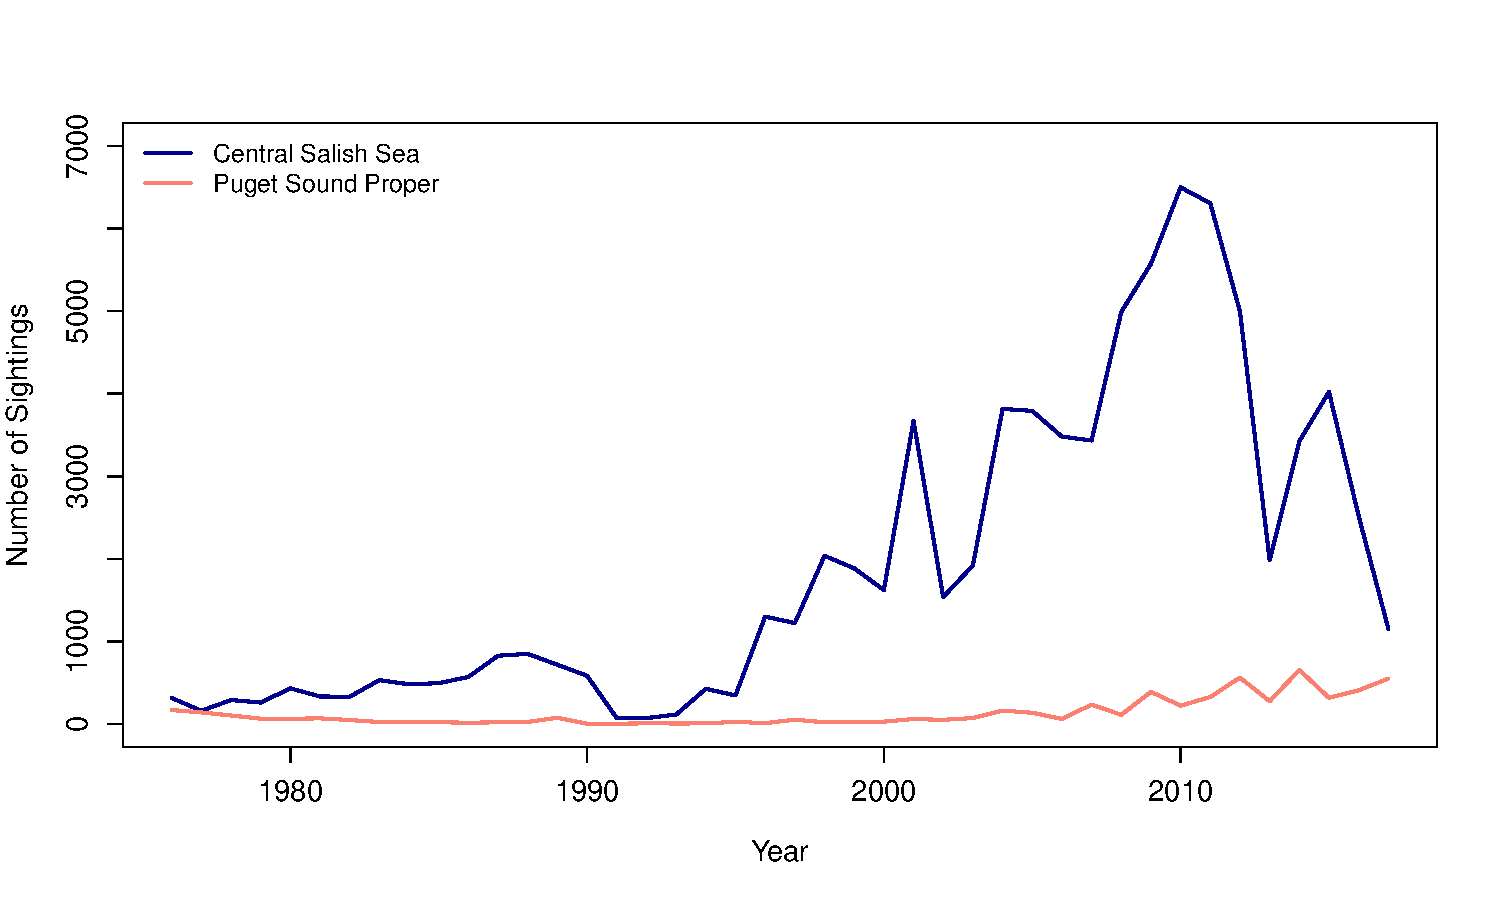
\includegraphics[width=0.8\textwidth]{../analyses/figures/OrcaPhenPlots/numsights_1976_2regs.pdf} 
\caption{\textbf{Sightings of SRKWs from the OrcaMaster Database}, from 1978-2017. }
\label{fig:sights}
\end{figure}

\begin{figure}[p]
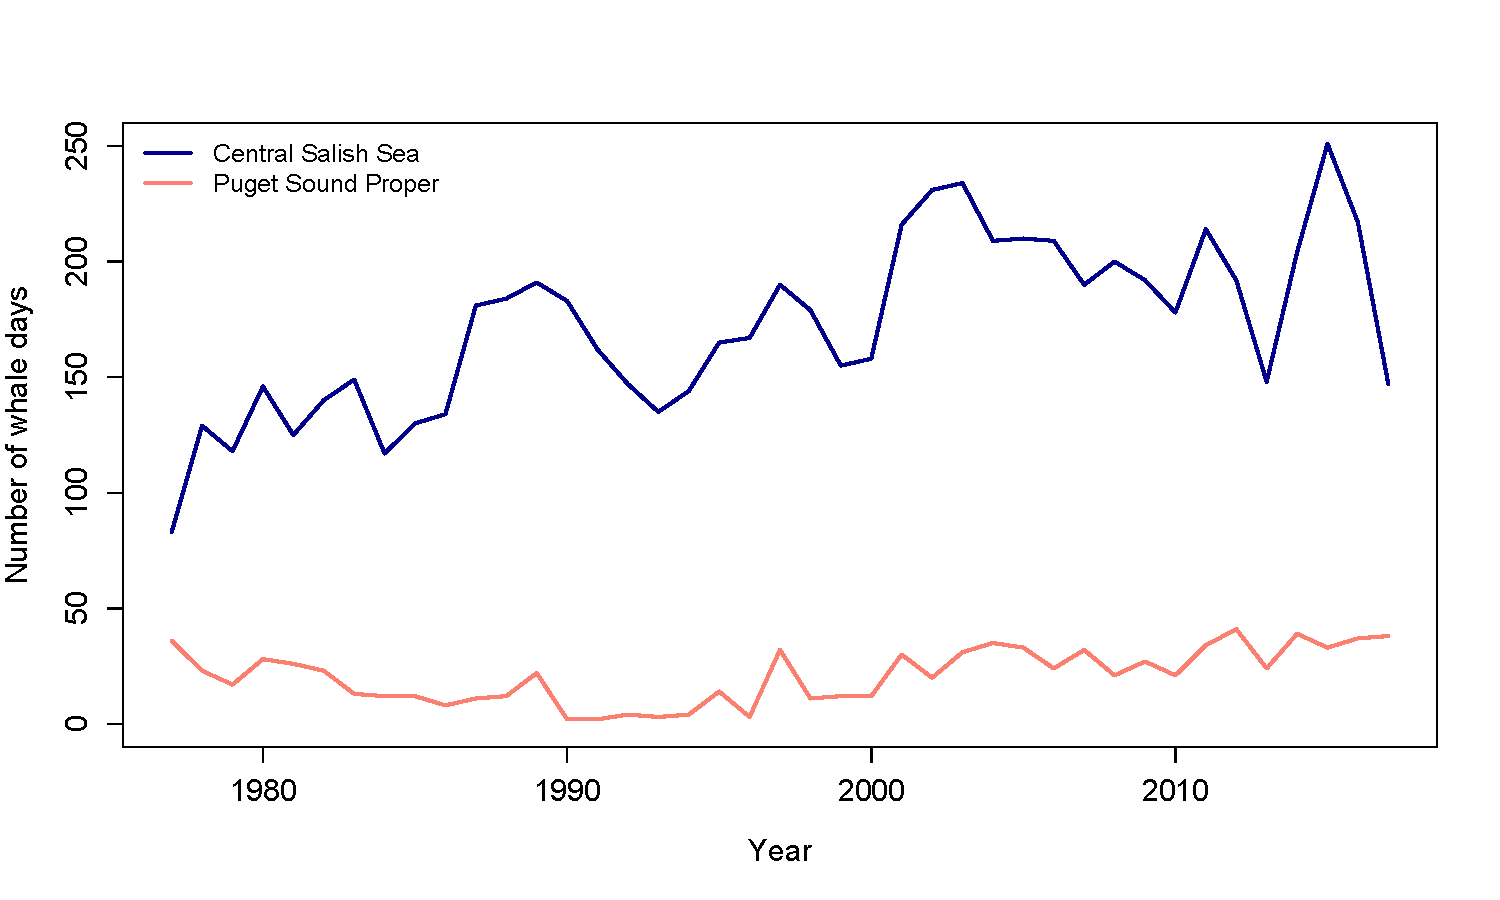
\includegraphics[width=0.8\textwidth]{../analyses/figures/OrcaPhenPlots/whaledays_assumeSRKW2regs.pdf} 
\caption{\textbf{Number of whale days from the OrcaMaster Database}, from 1978-2017. }
\label{fig:wdays}
\end{figure}

\begin{figure}[p]
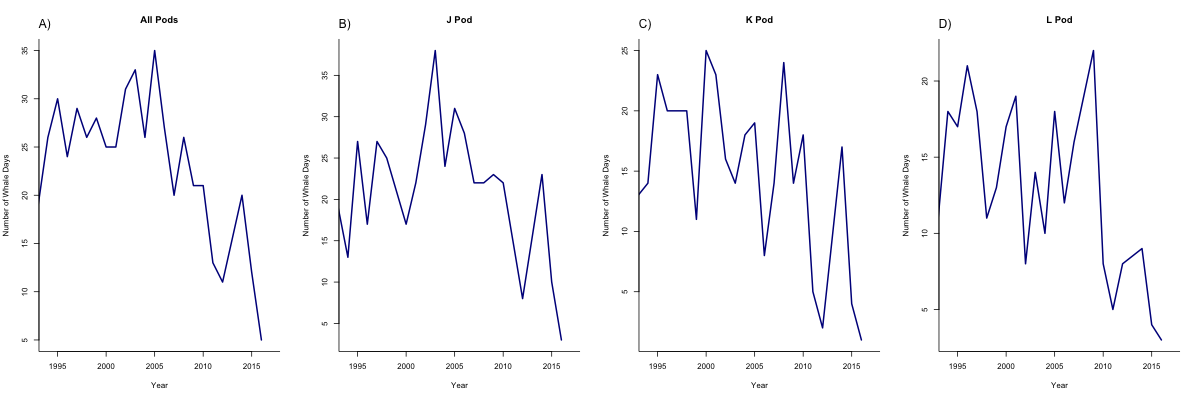
\includegraphics[width=0.8\textwidth]{../analyses/orcaphen/figures/whaledays_lime.png} 
\caption{\textbf{Number of whale days at Lime Kiln State Park} has declined since 1994, across all pods (A), J pod (B), K pod (C), and L pod (D). }
\label{fig:limewdays}
\end{figure}

\begin{figure}[p]
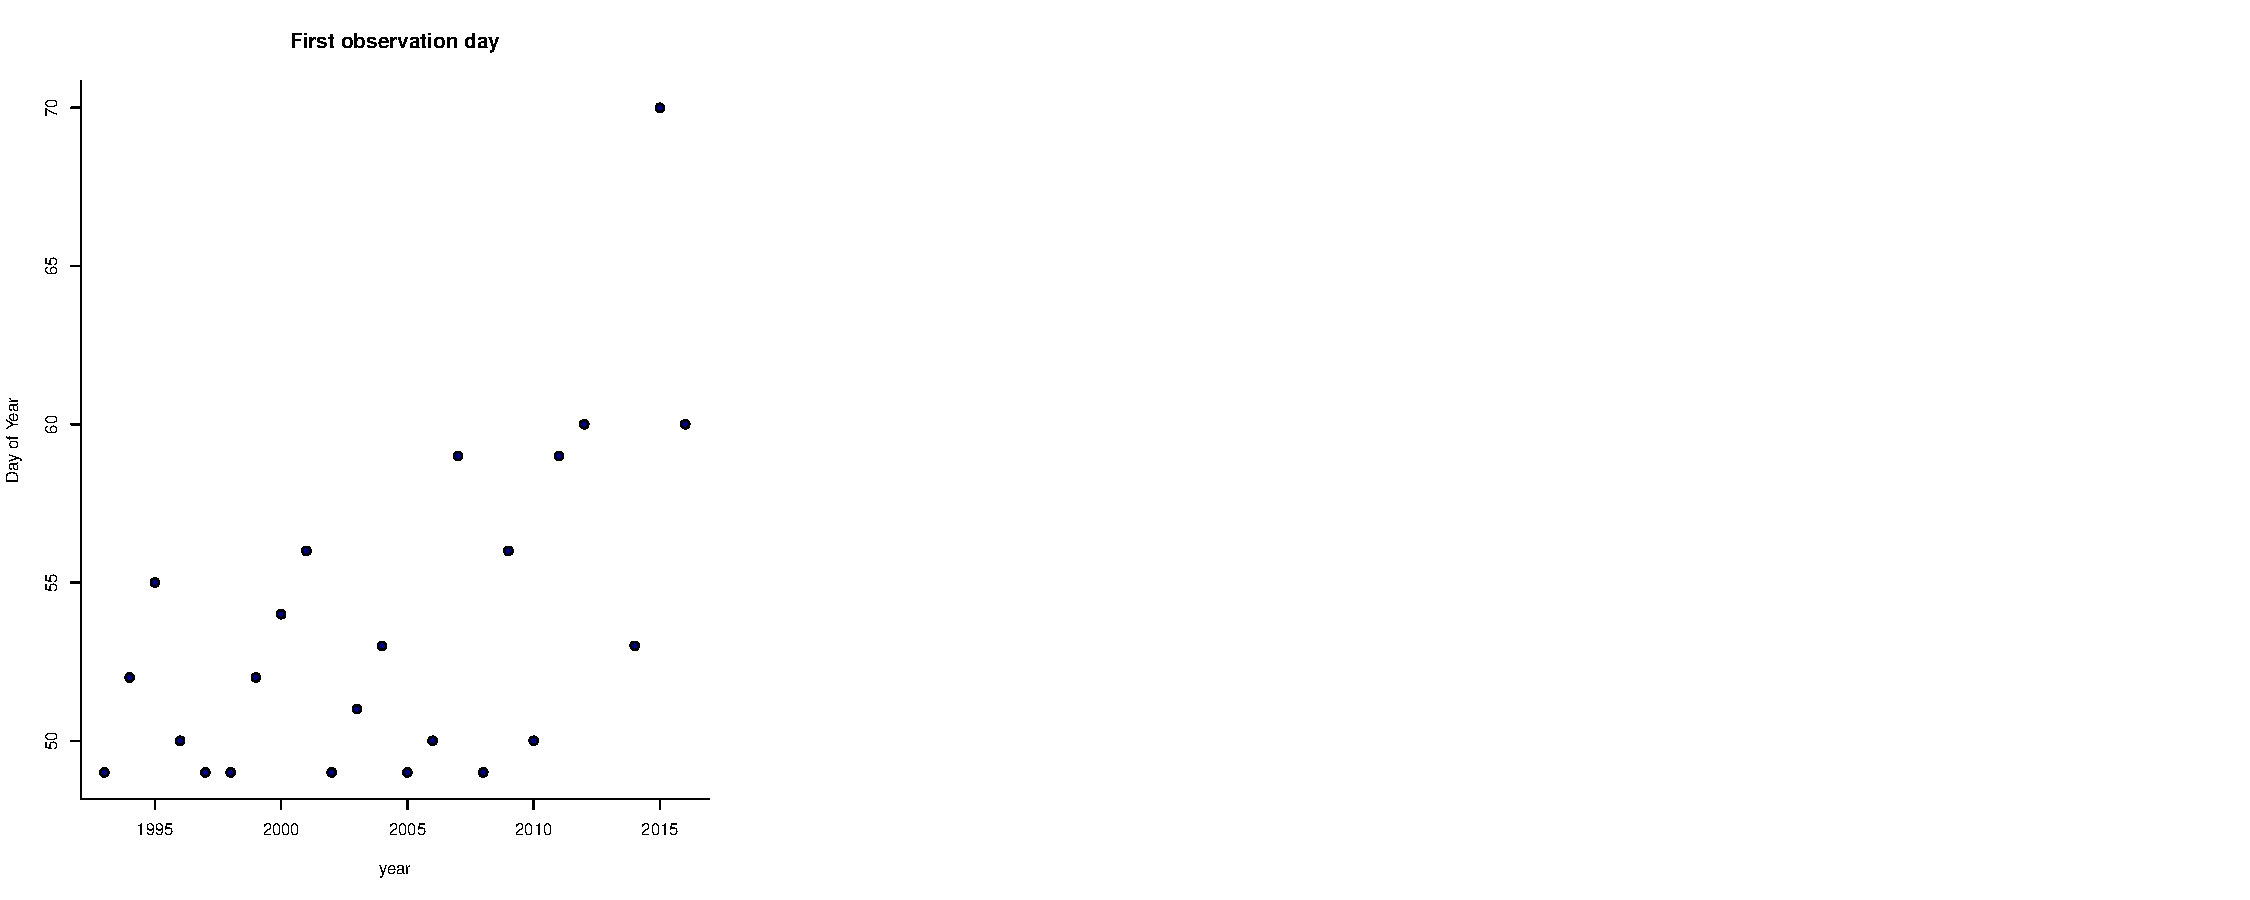
\includegraphics[width=0.8\textwidth]{../analyses/orcaphen/figures/limekilntrends_dat.pdf} 
\caption{\textbf{SRKW phenology at Lime Kiln State Park is shifting}, which the day of year of first sighting getting later (A) and the day of year of last sighting getting earlier frmo 1994-2017. These trends are associated with a decrease in the amount of time SRKWs are spending near Lime Kiln: the number of days on which SRKWs were observed ("whale days") has declined since 1994. }
\label{fig:limetime}
\end{figure}

\begin{figure}[p]
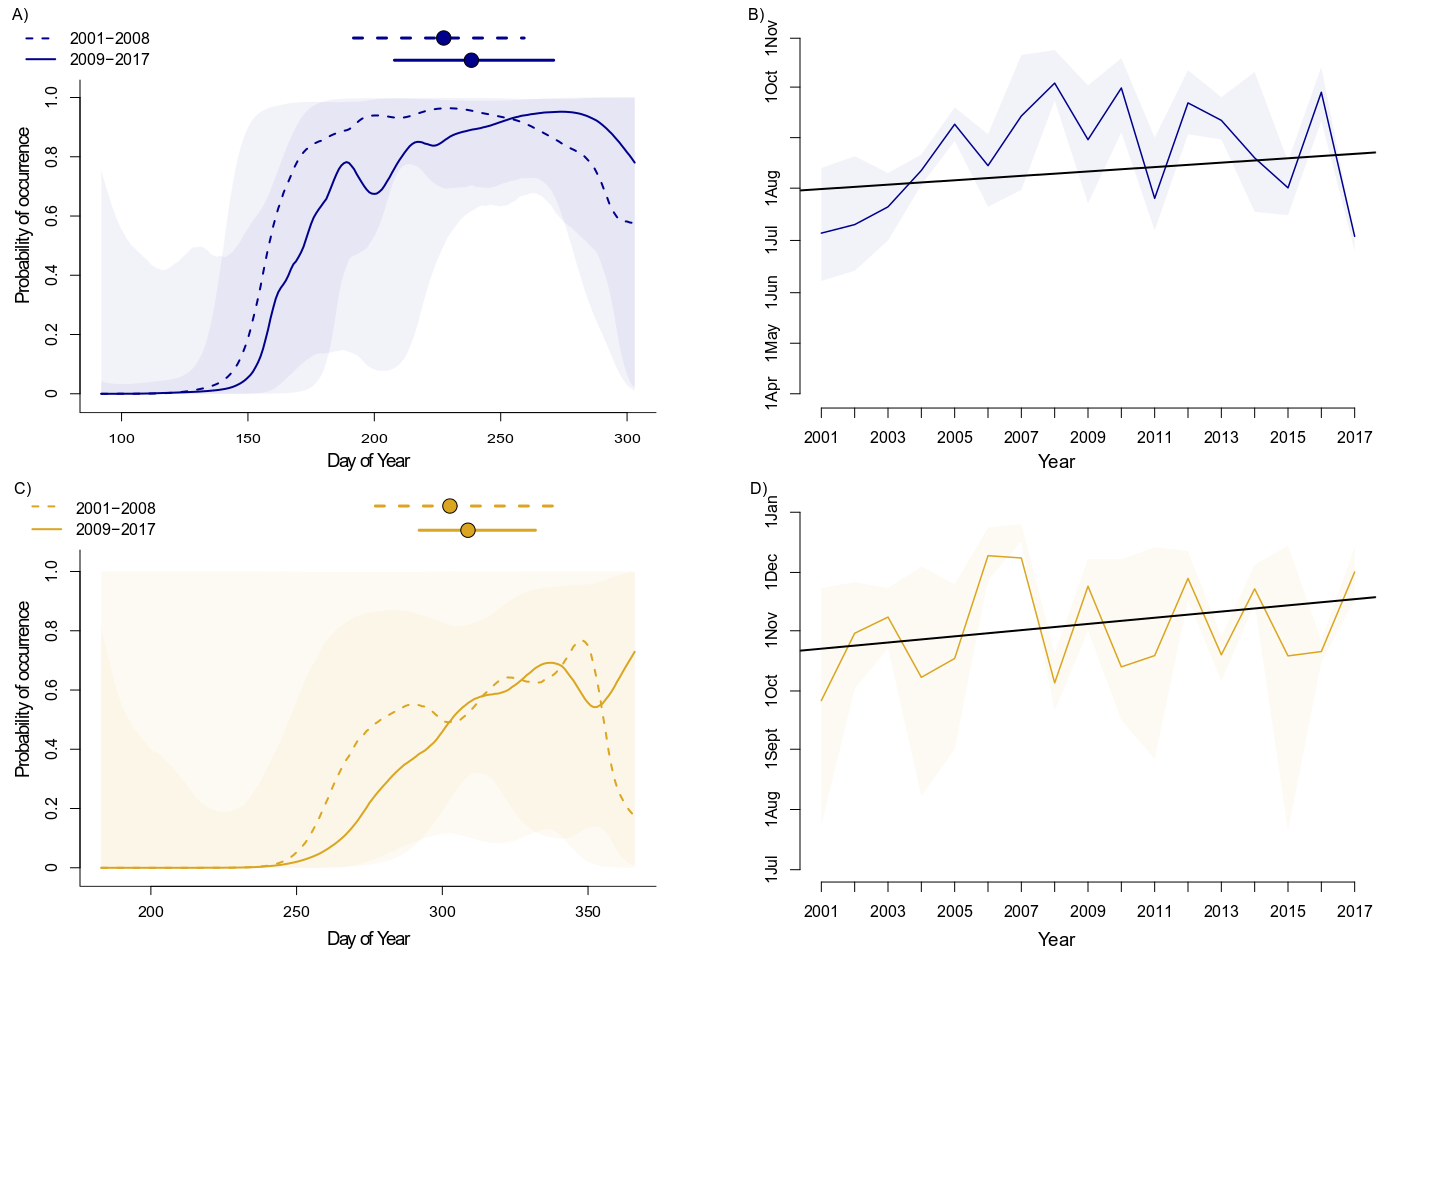
\includegraphics[width=0.8\textwidth]{../analyses/figures/proboccK_4panels.png} 
\caption{\textbf{K-pod activity varies seasonally in the Central Salish Sea (A) and Puget Sound proper (C).} This phenology has shifted later in recent years in the Central Salish Sea (B) and in Puget Sound (D). The shift toward later arrival in the central Salish Sea is evident the estimated probabilities of occurrence from the occupancy models for K-pod (A,C) as well as the linear trends in peak occurrence probability from 2001-2017 (B,D). Shading around lines represents 50\% credible intervals (95\% credible intervals in Table SX). 
}
\label{fig:Kprobs}
\end{figure}


\begin{figure}[p]
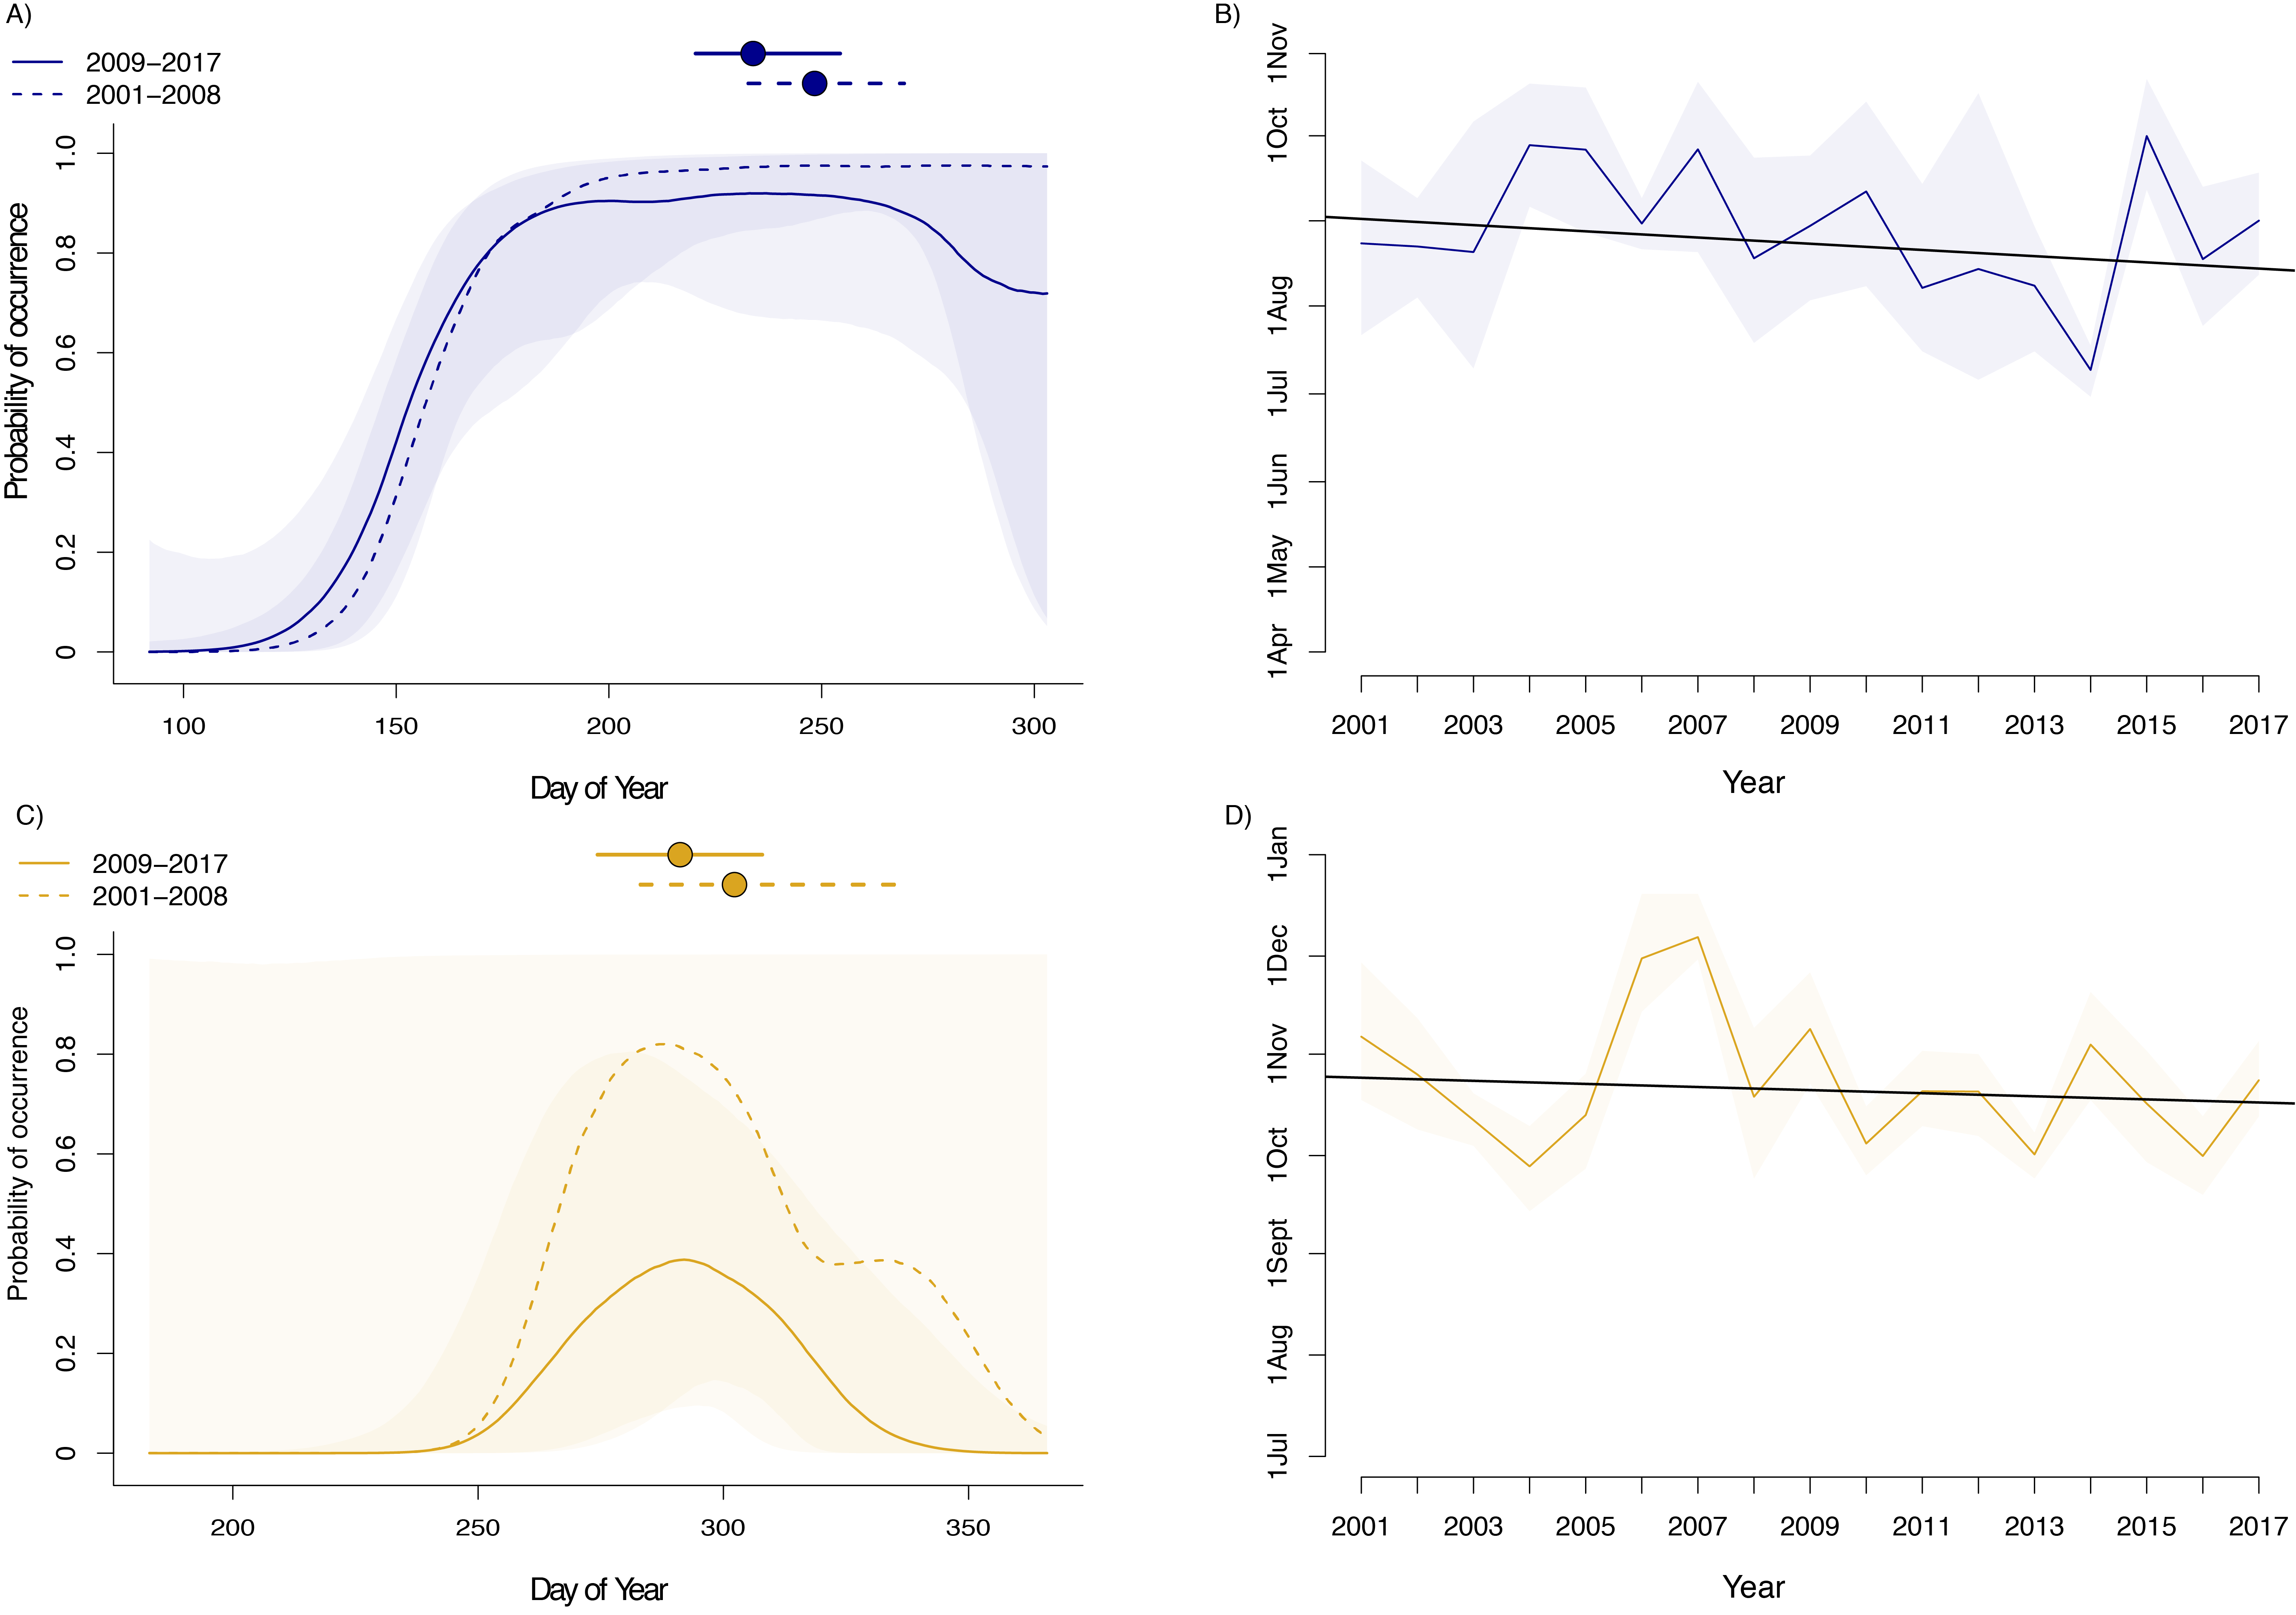
\includegraphics[width=0.8\textwidth]{../analyses/figures/proboccL_4panels.png} 
\caption{\textbf{L-pod activity varies seasonally in the Central Salish Sea (A) and Puget Sound proper (C)}. This phenology has shifted later in recent years in the Central Salish Sea (B) and in Puget Sound (D). The shift toward later arrival in the central Salish Sea is evident the estimated probabilities of occurrence from the occupancy models for K-pod (A,C) as well as the linear trends in peak occurrence probability from 2001-2017 (B,D). Shading around lines represents 50\% credible intervals (95\% credible intervals in Table SX). 
}
\label{fig:Lprobs}
\end{figure}
%Ailene’s To Do List
%Check #s and be consistent about CIs (95% in text,  50% in figures, both in supp)
%Notes for Discussion (possible points to add, from Meeting with Jameal and Chris):
%Phenology matters to killer whales in one region but not in other. Where it matters, things that modify timing should be included. Indirect to think about how hatchery timing could affect that. 
%Could reference atlantic modelling or scaling up to ecosystem level by referencing Isaac’s papers. Cite Lacey paper. On the other hand, you could regulate all the fishing and vessel traffic could still inhibit prey capture for SRKWs.
%Add a sentence for cumulative impacts on recovering prey . Try to think of other similar examples- perhaps on lands. Great barrier reef- taken one conservation action but another limiting factor in play. 
%Engage cumulative impacts, EBME literature to be broader. It's widely acknowledged %that cumulative impacts are threatening SRKWs. Timing is less often considered. %Will Satherwaite paper on salmon. Forecasting with SRKWs- managing 
%Disproportionate importance of some timing- Are there particular times of year  %when SRKWs are more sensitive to starvation (e.g. due to birth)? 
%Overall abundance is still important for prey.  But its not the whole story. %Phenology is not the whole story either.
%Fisheries are more direct way of managing prey than hatcheries.
%%%%%%%%%%%%%%%%%%%%%%%%%%%%%%%%%%%%%%
  \end{document}
%%%%%%%%%%%%%%%%%%%%%%%%%%%%%%%%%%%%%%
